\documentclass[10pt]{beamer}
%\usetheme[
%%% option passed to the outer theme
%    progressstyle=fixedCircCnt,   % fixedCircCnt, movingCircCnt (moving is deault)
%]{}
  
% If you want to change the colors of the various elements in the theme, edit and uncomment the following lines

% Change the bar colors:
%\setbeamercolor{Feather}{fg=red!20,bg=red}

% Change the color of the structural elements:
%\setbeamercolor{structure}{fg=red}

% Change the frame title text color:
%\setbeamercolor{frametitle}{fg=blue}

% Change the normal text color background:
%\setbeamercolor{normal text}{fg=black,bg=gray!10}

%-------------------------------------------------------
% INCLUDE PACKAGES
%-------------------------------------------------------

\usepackage[natbib=true,backend=bibtex,useprefix=true]{biblatex}
\addbibresource{bibliography.bib}
\usepackage[utf8]{inputenc}
\usepackage{quoting}
\usepackage{tikz}
\usepackage{ragged2e}
\usepackage{adjustbox}
\justifying

%-------------------------------------------------------
% DEFFINING AND REDEFINING COMMANDS
%-------------------------------------------------------

\usetheme{Warsaw}

%-------------------------------------------------------
% INFORMATION IN THE TITLE PAGE
%-------------------------------------------------------

\title[] % [] is optional - is placed on the bottom of the sidebar on every slide
{ % is placed on the title page
      \textbf{Characterizing and Classifying IoT Traffic in Smart Cities and Campuses}
}

\subtitle[]
{
      \textbf{Paper's analysis\\ITPA 2019-2020}
}

\author[Andrea Graziani - 0273395]
{      Andrea Graziani - 0273395 \\
      {}
}

\institute[]
{
      Università degli Studi di Roma “Tor Vergata” \\
      FACOLTA' DI INGEGNERIA \\
      Corso di Laurea Magistrale in Ingegneria Informatica
  
  %there must be an empty line above this line - otherwise some unwanted space is added between the university and the country (I do not know why;( )
}

\date{\today}

%-------------------------------------------------------
% THE BODY OF THE PRESENTATION
%-------------------------------------------------------

\begin{document}

%-------------------------------------------------------
% THE TITLEPAGE
%-------------------------------------------------------

{% % this is the name of the PDF file for the background
\begin{frame}[plain,noframenumbering] % the plain option removes the header from the title page, noframenumbering removes the numbering of this frame only
  \titlepage % call the title page information from above
\end{frame}}


\section{Introduction}
\subsection{Research's goal}
%---------------------------------------------------------------------------------------------------------%
\begin{frame}{Research's goal}
%---------------------------------------------------------------------------------------------------------%

According to \citet{ITPAReport}, research's goal is to:

\begin{quoting}[font=itshape, begintext={``}, endtext={''}]
[...] develop a classification method that can not only distinguish IoT from non-IoT traffic, but also identify specific IoT devices with over 95\% accuracy.
\end{quoting}

\begin{alertblock}{\textbf{What is the reason according to which is important to profile IoT traffic?}}
\justifying
\begin{enumerate}
\justifying
\item To understand IoT devices ``\textit{normal}" \textbf{traffic pattern} in terms of their \textbf{activity pattern} (traffic rate, idle durations, etc.) and \textbf{signalling overheads} (\texttt{DNS}, \texttt{NTP}, etc.). 

\item To enhance \textbf{cyber-security} involving IoT devices which administration belong to \textbf{different authorities}. 

According to \citet{ITPAReport}, is possible to improve security deploying a network-level security mechanisms which, analysing traffic patterns, is capable to \textbf{identify attacks knowing the normal traffic pattern of monitored IoT devices}.

\end{enumerate}

\end{alertblock}


%---------------------------------------------------------------------------------------------------------%
\end{frame} 
%---------------------------------------------------------------------------------------------------------%

%---------------------------------------------------------------------------------------------------------%
\begin{frame}{Research's goal}
%---------------------------------------------------------------------------------------------------------%

In other words, research's goal is to build an classification model for IoT devices based on \textbf{machine learning} techniques, which building passes through following steps:

\begin{enumerate}
\item Collect data from an IoT environment.
\item Characterize traffic pattern corresponding to the various IoT devices.
\item Develop a classification technique that learns the behaviour of an IoT device and is able to identify it based on its traffic pattern.
\end{enumerate}



We believe that the ``Smart environment" by researchers is not suitable for to build an IoT traffic trace in order to classifiyn IoT traffic in smart cities and campuses for security purposes.

We are convinced that model not 

Due to the \textbf{type} and the \textbf{number} (only $20$ devices!) of IoT devices used for their experiments, adopted ``Smart environment" is more suitable for a smart home rather than a smart city or campus as stated by authors.




%---------------------------------------------------------------------------------------------------------%
\end{frame} 
%---------------------------------------------------------------------------------------------------------%
\section{Dataset building}
%---------------------------------------------------------------------------------------------------------%
\begin{frame}{Data-set building}{\justifying}
%---------------------------------------------------------------------------------------------------------%

\begin{itemize}

\item Since \citet{ITPAReport} adopted a \textbf{supervised machine learning algorithms} to build their model, is necessary to generate a \textbf{data-set}, in order to provide an appropriate input for the \textbf{learning phase}.


\end{itemize}

To be precise, \citet{ITPAReport} built a \textbf{time series} dataset, where each instance is indexed by time.

Each data-set's instance contain following \textbf{attributes} (or \textbf{features}):
\begin{itemize}
\item Traffic load.
\item Average packet size
\item Protocol used and port number
\item active and sleep times
\item unique DNS requests, 
\item NTP interval, 
\item peak/mean rate
\end{itemize}

%---------------------------------------------------------------------------------------------------------%
\end{frame} 
%---------------------------------------------------------------------------------------------------------%
\subsection{``Smart environment"'s analysis}
%---------------------------------------------------------------------------------------------------------%
\begin{frame}{``Smart environment"'s analysis: Overview}
%---------------------------------------------------------------------------------------------------------%

In order to building needed dataset, simulating a real usage scenario, \citet{ITPAReport} built a so-called ``\textit{smart environment}", including:

\begin{itemize}
\justifying
\item $21$ unique IoT devices representing different categories, like \textbf{cameras}, \textbf{healthcare devices}, \textbf{hub}, \textbf{air quality sensors} and so on.

\item A router, the \textsc{TP Link Archer C7}\footnote{\tiny\url{https://www.tp-link.com/it/home-networking/wifi-router/archer-c7/\#overview}}

\item Several non-IoT devices were also used, such as laptops, mobile phones and tablet.

\end{itemize}

\begin{figure}
  \caption{``Smart environment"'s scheme}
  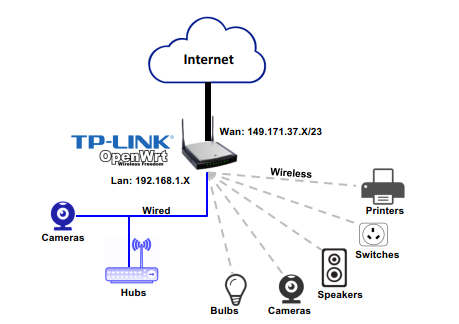
\includegraphics[width=100pt]{Topology.png}
\end{figure}

%---------------------------------------------------------------------------------------------------------%
\end{frame} 
%---------------------------------------------------------------------------------------------------------%
%---------------------------------------------------------------------------------------------------------%
\begin{frame}{``Smart environment"'s analysis: Observations}
%---------------------------------------------------------------------------------------------------------%

\begin{alertblock}{Observation \# 1}
The experimental smart environment build by researchers is characterized by a \textbf{star network topology}.
\end{alertblock}

This is a very important observation, because a star topology allows us to:

\begin{itemize}
\justifying
\item \textbf{Preserve battery life} of IoT devices because they \textbf{do not have to forward} other nodes data; in other words, \textit{any IoT device receives, or transmits, only its own data}.

\item \textbf{Decrease the complexity} of the network.
\end{itemize}

\begin{block}{The LPWAN example}
\justifying
The implementation of \texttt{LoRaWAN} network is based on the star network topology, and mostly, stars-of-stars network. 

As known \texttt{LoRaWAN} network belongs to \texttt{LPWAN} category, \textit{which are specifically designed to achieve the need for low power, long-range, low bit error rate, and low cost} needed in IoT context. 
\end{block}

%---------------------------------------------------------------------------------------------------------%
\end{frame} 
%---------------------------------------------------------------------------------------------------------%
%---------------------------------------------------------------------------------------------------------%
\begin{frame}{``Smart environment"'s analysis: Observations}
%---------------------------------------------------------------------------------------------------------%

\begin{alertblock}{Observation \# 2}
Researchers use \texttt{IEEE 802.11} as \textbf{media access control} (\texttt{MAC}) and \textbf{physical layer} (\texttt{PHY}) protocol.
\end{alertblock}

\begin{alertblock}{Observation \# 3}
Researchers did \textit{not} specify which \textbf{version} of IEEE 802.11 standard has been effectively used. 

We don't know with which \textbf{frequencies} data has been transmitted.
\end{alertblock}

According to vendor's specifications regarding the \textsc{TP Link Archer C7}, is possible to know that the aforementioned router supports following protocols:

\begin{itemize}
\item \texttt{IEEE 802.11ac/n/a} at $5$ GHz
\item \texttt{IEEE 802.11n/b/g} at $2.4$ GHz
\end{itemize}

%---------------------------------------------------------------------------------------------------------%
\end{frame} 
%---------------------------------------------------------------------------------------------------------%
%---------------------------------------------------------------------------------------------------------%
\begin{frame}{``Smart environment"'s analysis: Observations}
%---------------------------------------------------------------------------------------------------------%

\begin{alertblock}{Observation \# 4}
\justifying
We believe that above protocols are \textbf{not} fully optimized for IoT business models and devices used in smart cities and campuses for following reasons:

\begin{itemize}
\justifying
\item These technologies provide a \textbf{short/medium coverage} with \textbf{100-to-1000} meters range. Provided coverage range can be not enough to fulfil all use cases.

\begin{itemize}
\item This is due to \textbf{mid/high frequencies} used by these protocol which are \textbf{vulnerable to several side effect during signal propagation} (\textit{blocking}, \textit{reflection}, \textit{refraction} and so on)
\end{itemize}


\item As stated by \citet{ITPAReport} too, IoT devices require \textbf{low power} and less \textbf{data-rate}.

\item They are affected by overhead caused by short packets transmission which are very common is many IoT scenarios.

\end{itemize}
\end{alertblock}


%---------------------------------------------------------------------------------------------------------%
\end{frame} 
%---------------------------------------------------------------------------------------------------------%
%---------------------------------------------------------------------------------------------------------%
\begin{frame}{``Smart environment"'s analysis: Observations}
%---------------------------------------------------------------------------------------------------------%

\begin{block}{}
\justifying
Utilizing sub-1 GHz bands used \texttt{802.11ah} or \texttt{LoRaWAN} by to provide better propagation characteristics in outdoor scenarios. Low frequencies signal are less affected by obstacles presence.
\end{block}

\begin{block}{}
A combination of low-band, mid-band and high-band spectrum is desirable to manage all possible use cases.
\end{block}

\begin{adjustbox}{width=\columnwidth,center}
\begin{tabular}{l|ccccc}

& \textbf{802.11ac} & \textbf{802.11n} & \textbf{802.11a} & \textbf{802.11ah} & \textbf{LoRaWAN} \\
\hline
\textbf{Frequency (GHz)} & $5$ & $2.4$,$5$ & $5$ & $0.7/0.8/0.9$ & $0.863-8.70 (EU)$ \\
\textbf{Sensitivity (dbm)} & $-82$ & $-82$ & $-88$ & $-98$ &  $[-124,-137]$ \\
\textbf{Bit rate (Mb/s)} & $6.5$ & $6.5$ & $1.5$ & $0.15$ & $[293, 5469]$ \\
\textbf{Max coverage range (km)} &&&& $\backsim 1$ & $\backsim 15$ \\

\end{tabular}
\end{adjustbox}


%---------------------------------------------------------------------------------------------------------%
\end{frame} 
%---------------------------------------------------------------------------------------------------------%
\subsection{IoT Traffic}
%---------------------------------------------------------------------------------------------------------%
\begin{frame}{IoT Traffic}
%---------------------------------------------------------------------------------------------------------%

According to their experimental results, \citet{ITPAReport} stated that:

\begin{quoting}[font=itshape, begintext={``}, endtext={''\cite[par.~IV.A]{ITPAReport}}]
\justifying
[...] if we consider only the load imposed by the IoT devices, then there is a dramatic reduction in the peak load ($1$ Mbps) and average loads ($66$ Kbps), [...], implying that traffic generated by IoT devices is small compared to traditional non-IoT traffic. 
\end{quoting}

\begin{quoting}[font=itshape, begintext={``}, endtext={''\cite[par.~IV.A]{ITPAReport}}]
\justifying
the traffic pattern of one IoT device [...] a pattern of active/sleep communication emerges. [...] IoT active time [...] decays rapidly initially (only 5\% of sessions last longer than 5 seconds), with the maximum active time being 250 seconds in our trace. This shows that IoT activities are short-lived in general. 
\end{quoting}


%---------------------------------------------------------------------------------------------------------%
\end{frame} 
%---------------------------------------------------------------------------------------------------------%

%---------------------------------------------------------------------------------------------------------%
\begin{frame}{}
%---------------------------------------------------------------------------------------------------------%

\begin{block}{Observation \# 1}
Several IoT devices used by \citet{ITPAReport} for their experiments \textbf{are battery operated}. 

For instance:

\begin{itemize}
\item The \textit{Withings Smart scale} device is powered by $4$ $1.5$ \textit{V} alkaline cells (AAA).\footnote{\url{https://www.withings.com/it/en/body}}

\item Similarly, the \textit{Netatmo Weather station} device is powered by $2$ $1.5$ \textit{V} alkaline cells (AAA) with an \textbf{estimated autonomy of about 2 years}.\footnote{\url{https://www.netatmo.com/it-it/weather/weatherstation/specifications}
}
\item The \textit{Blipcare blood pressure meter} device is powered by an internal battery.\footnote{\url{http://www.blipcare.com/}}
\end{itemize} 

\end{block}

%---------------------------------------------------------------------------------------------------------%
\end{frame} 
%---------------------------------------------------------------------------------------------------------%


%---------------------------------------------------------------------------------------------------------%
\begin{frame}{}
%---------------------------------------------------------------------------------------------------------%

\begin{block}{}
Since many IoT devices are battery powered, \textbf{maximize energy efficiency}, in order to \textbf{preserve devices lifetime}, is critical. 
\end{block}

\begin{block}{}
As expected, observing the figure reported below, is very easy to understand that the power management approach, used to preserve battery life, is based on \textbf{periodic sleep}, during which radio transceiver are turned off.
\end{block}

\begin{figure}
  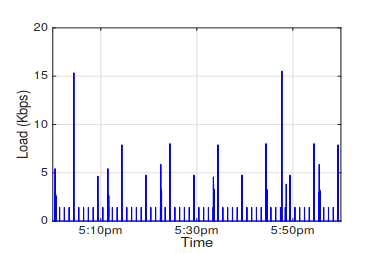
\includegraphics[width=150pt]{SleepTime.png}
  \caption{Load of LiFX light bulb device.}
  \label{fig1}
\end{figure}

%---------------------------------------------------------------------------------------------------------%
\end{frame} 
%---------------------------------------------------------------------------------------------------------%



\section{IoT Application Layer Protocol}
\subsection{Security issues}
%---------------------------------------------------------------------------------------------------------%
\begin{frame}{}
%---------------------------------------------------------------------------------------------------------%
\begin{itemize}

\item According to \citet{ITPAReport}'s report, 

\vspace{0.3cm}
\begin{quoting}[font=itshape, begintext={``}, endtext={''\cite[par.~IV.B]{ITPAReport}}]
Nevertheless, about 45\% of IoT traffic (by number of packets) is not sent over \texttt{HTTPS} to the servers on the public Internet indicating that a sizeable fraction of IoT traffic is not being securely transported over the Internet.
\end{quoting}
\vspace{0.3cm}

Another challenge facing IoT successful deployment is the
lack of a universal platform, protocol, and a programming
language. Today, all connected devices follow a different set
of protocols and platforms. The need of the time is to have
collaboration among the connecting devices. For this, large
enterprises such as LG, Samsung and Philips etc. should join
hands and make a consortium for the development of universal coding language and platform. The proposed solution
can solve the compatibility issues of IoT up to a significant
extent



\end{itemize}
%---------------------------------------------------------------------------------------------------------%
\end{frame} 
%---------------------------------------------------------------------------------------------------------%





%---------------------------------------------------------------------------------------------------------%
\begin{frame}{}
%---------------------------------------------------------------------------------------------------------%


Another challenge facing IoT successful deployment is the
lack of a universal platform, protocol, and a programming
language. Today, all connected devices follow a different set
of protocols and platforms. The need of the time is to have
collaboration among the connecting devices. For this, large
enterprises such as LG, Samsung and Philips etc. should join
hands and make a consortium for the development of universal coding language and platform. The proposed solution
can solve the compatibility issues of IoT up to a significant
extent

%---------------------------------------------------------------------------------------------------------%
\end{frame} 
%---------------------------------------------------------------------------------------------------------%


\subsection{Why HTTP/HTTPS is so important? issues}
%---------------------------------------------------------------------------------------------------------%
\begin{frame}{}
%---------------------------------------------------------------------------------------------------------%
\begin{itemize}

\item Why \texttt{HTTPS} and \texttt{HTTP} are the dominant protocols used by IoT devices, as stated by \citet{ITPAReport}?

\begin{itemize}
\item As stated by \citet{WOT}, HTTP/HTTPS protocols play a very important role into \textbf{Web of Things Architecture} for several reasons:
\begin{enumerate}
\item Facilitate both the \textbf{integration of IoT devices} with existing services currently available on the Web and the  \textbf{Web applications development} exploiting \textbf{REST architectural style}

\item They offer a \textbf{direct access} for users to IoT devices data and services, without the need for installing additional software. 

In fact, using a Web browser (or any HTTP library in the case of a software client) client are able to to directly extract, save and share smart things data and services. 

This ensures the usability of the architecture and minimizes the entry barriers for final users.
\end{enumerate}



\end{itemize}

\end{itemize}
%---------------------------------------------------------------------------------------------------------%
\end{frame} 
%---------------------------------------------------------------------------------------------------------%



%---------------------------------------------------------------------------------------------------------%
\begin{frame}{}
%---------------------------------------------------------------------------------------------------------%
\begin{itemize}

\item According to \citet{ITPAReport}, the set of IoT devices used for their experiments including a huge amount of \textbf{sensors}, including air quality sensors and health-care devices. 

As known, aforementioned kind of devices generate a huge amount of data modelled as \textbf{time series}, that is an array of values indexed by time. 

According to \citet{TIMESERIES}, the stream of data generated by all these IoT sensors is generally interfaced with database, through a so-called \textit{southbound} interface, using HTTP RESTful protocol. Similarly, all applications requiring access to the data stored in the database, using the same protocol, through a so-called northbound interface. 

\end{itemize}
%---------------------------------------------------------------------------------------------------------%
\end{frame} 
%---------------------------------------------------------------------------------------------------------%









\begin{frame}[noframenumbering,shrink=15]{Some references}
\printbibliography
\end{frame}
\end{document}
